%%%%%%%%%%%%%%%%%%%%%%%%%%%%%%%%%%%%%%%%%%%%%%%%%%%%%%%
% Please note that whilst this template provides a
% preview of the typeset manuscript for submission, it
% will not necessarily be the final publication layout.
%
% letterpaper/a4paper: US/UK paper size toggle
% num-refs/alpha-refs: numeric/author-year citation and bibliography toggle

%\documentclass[letterpaper]{oup-contemporary}
\documentclass[a4paper,num-refs]{oup-contemporary}

%%% Journal toggle; only specific options recognised.
%%% (Only "gigascience" and "general" are implemented now. Support for other journals is planned.)
\journal{gigascience}

\usepackage{graphicx}
\usepackage{siunitx}
\usepackage{listings}

%%% Flushend: You can add this package to automatically balance the final page, but if things go awry (e.g. section contents appearing out-of-order or entire blocks or paragraphs are coloured), remove it!
% \usepackage{flushend}

\title{Training Infrastructure as a Service}

%%% Use the \authfn to add symbols for additional footnotes, if any. 1 is reserved for correspondence emails; then continuing with 2 etc for contributions.
\author[1,1a\authfn{1}]{Helena~Rasche}
\author[2]{Cameron~Hyde}
\author[3]{John~Davis}
\author[4]{Simon~Gladman}
\author[5]{Nate~Coraor}
\author[6]{Anthony~Bretaudeau}
\author[7]{Gianmauro~Cuccuru}
\author[1]{Saskia Hiltemann}
\author[8]{Beatriz Serrano-Solano}
\author[9]{Jennifer~Hillman-Jackson}
\author[10\authfn{2}]{Bj\"orn~Gr\"uning}
\author[1\authfn{2}]{Andrew~Stubbs}

\affil[1]{Clinical Bioinformatics Group, Department of Pathology, Erasmus Medical Center, Wytemaweg 80, 3015 CN, Rotterdam, The Netherlands}
\affil[1a]{Academie voor de Technologie van Gezondheid en Milieu, Avans Hogeschool, Lovensdijkstraat 63, 4818 AJ Breda, the Netherlands}
\affil[2]{Cam Affil}
\affil[3]{John D Affil}
\affil[4]{Simon G Affil}
\affil[5]{Nate C Affil}
\affil[6]{Anthony B Affil}
\affil[7]{Gianmauro C Affil}
\affil[8]{Bea S-S Affil}
\affil[9]{Jen H-J Affil}
\affil[10]{Bioinformatics Group, Department of Computer Science, University of Freiburg, 79110 Freiburg im Breisgau, Germany}

%%% Author Notes
\authnote{\authfn{1}e.rasche@erasmusmc.nl}
\authnote{\authfn{2}These authors contributed equally.}

%%% Paper category
\papercat{Technical Note}

%%% "Short" author for running page header
\runningauthor{Rasche et al}

%%% Should only be set by an editor
\jvolume{00}
\jnumber{0}
\jyear{2020}

\begin{document}

\begin{frontmatter}
\maketitle
\begin{abstract}
%The Abstract (250 words maximum) should be structured to include the following details: \textbf{Background}, the context and purpose of the study; \textbf{Results}, the main findings; \textbf{Conclusions}, brief summary and potential implications. Please minimize the use of abbreviations and do not cite references in the abstract.
\textbf{Background:} Hands-on training, whether in bioinformatics or other domains, often requires significant technical resources and knowledge to set up and run.
Instructors must have access to powerful compute infrastructure that can support resource-intensive jobs running efficiently.
Often this is achieved using a private server where there is no contention for the queue. However, this places a significant pre-requisite knowledge or labour barrier for teachers, who must spend time coordinating deployment and management of compute resources. In addition, with the increase of virtual and hybrid teaching, where learners are located in separate physical locations, it is difficult to track student progress as efficiently as during in-person courses.

\textbf{Findings:} Originally developed by Galaxy Europe and the Gallantries project, together the Galaxy community we have created Training-Infrastructure-as-a-Service (TIaaS), aimed at providing user-friendly training infrastructure to the global training community. TIaaS provides free, dedicated training resources for Galaxy-based courses and events. Event organisers must register their course, after which trainees are transparently placed in a private queue on the compute infrastructure, which ensures jobs complete quickly, even when the main queue is experiencing high wait times. Additionally, instructors can monitor student progress via the built-in dashboard.

\textbf{Conclusions:} TIaaS provides a significant improvement for instructors and learners, as well as infrastructure administrators. The instructor dashboard makes remote events not only possible but easy. Students experience continuity of learning, as all training happens on the public Galaxy which they can continue to use after the event. In the past 48 months, $>360$ training events with over 18,000 learners have used this infrastructure for Galaxy training.
\end{abstract}

\begin{keywords}
Galaxy; Training; Teaching; Remote Training
\end{keywords}
\end{frontmatter}

\section{Findings}
\subsection{Background}

% The background section should be written in a way that is accessible to researchers without specialist knowledge in that area and must clearly state---and, if helpful, illustrate---the background to the research and its aims. The section should end with a brief statement of what is being reported in the article.

With the large volume of bioinformatics data becoming available, the availability of training for bioinformaticians and data scientists is not keeping up, resulting in a training gap \cite{Attwood2017}.
The Galaxy platform \cite{afgan2018galaxy} provides infrastructure on which to not only perform data analysis, but also conduct trainings, as it provides a user-friendly web-based interface to command-line analysis tools. Teaching with Galaxy significantly decreases infrastructure preparation time for instructors. With a wide range of tools (8000+) across a wide range of scientific domains, and pre-existing popularity within the life sciences community, Galaxy is an ideal platform for training \cite{gtn}.

In an attempt to address the training gap, the Galaxy community has, over the past several years, developed a wide array of hands-on tutorials (275+), covering bioinformatics and beyond, and made these materials FAIR \cite{Wilkinson2016-zo,10.1371/journal.pcbi.1007854}, and publicly available on the Galaxy Training Network (GTN) repository \cite{training-site}. In order to run these tutorials at scale, one often needs access to significant resources. For example, the GTN's most popular tutorial, ``Reference-based RNA-Seq data analysis'', uses the STAR aligner \cite{Dobin2012}. While such an ultra-fast aligner is ideal during training, as it reflects real-world analysis, it also consumes $\approx$32 GB of RAM at minimum\footnote{It uses 90Gb in the default configuration on UseGalaxy.eu. Many tools have similar requirements; on UseGalaxy.eu, 83 tools require $>$64 GB RAM, 151 require more than $>$32 GB, a limiting factor especially for smaller training infrastructures. Even with a large cluster, large class sizes can still consume all of the available overhead.}. While individual STAR jobs might execute successfully, the infrastructure remains a limiting factor for events with large number of participants that wish to stick to a schedule. When jobs must queue due to throughput limitations, this significantly impacts a training's timeline to the detriment of learners. While the instructor could alternatively deploy their own private infrastructure, this requires significant additional knowledge, time, energy, and funds. All of which are significant barriers for bioinformatics instructors trying to share their knowledge.

The training events hosted as part of the Gallantries project \cite{gallantries}, were the first foray into hybrid training for UseGalaxy.eu instructors. In hybrid training, one main instructor teaches in front of a camera, and this feed is live-streamed to multiple satellite classrooms, in geographically distinct locations. Each satellite location has on-site helpers present to support students and provide communication back to the main instructor. During one of the initial Gallantries hybrid training events--wherein we had three classrooms spread across the Netherlands, Germany, and Greece--we discovered that staying updated on student progress was a significant pain point. Normally teachers of hands-on lessons tend to wander around the classroom to check that students are not encountering difficulties, or use the Carpentries-style \cite{thecarpentries,Wilson2016} method of red and green sticky notes to let students communicate whether things are going well or poorly. In hybrid events this progress tracking is more difficult as on-site staff need to survey the room and report back centrally to the teacher, and is near impossible in fully remote training events such as have been more prevalent during the last 3 years of the pandemic.

\subsection{Results}

We initially developed Training Infrastructure as a Service (TIaaS) to solve our primary problems of ensuring we could quickly setup dedicated training resources which would be private to a single course. By re-using an existing public server backed by significant compute resources, we completely remove the infrastructure setup and maintenance costs of hosting an event for instructors. This centralisation also reduces the infrastructure requirements, as training events are rarely concurrent and can share the same hardware when not running simultaneously. 

The TIaaS system can be deployed on any Galaxy server, and is flexible, allowing Galaxy administrators to customize the settings to fit their needs and compute infrastructure. TIaaS is currently deployed on all 3 major Galaxy servers (Galaxy EU, Galaxy Australia, and Galaxy US), and numerous other smaller servers in public and private deployments. While individual TIaaS deployments can handle job scheduling differently, they generally allocate private resources so jobs can always run without delay. TiaaS provides good separation of responsibilities between instructors who are teaching and the server administrators responsible for Galaxy, rather than requiring instructors to be cross-trained in server administration. The live dashboard (Figure \ref{figure:dashboard}) showing participant jobs provides visibility into student progress and enables instructors to flag potential issues that may benefit from additional discussion with learners. We have shared this service with the Galaxy training community to overwhelmingly positive feedback.

\begin{figure}[bt!]
\centering
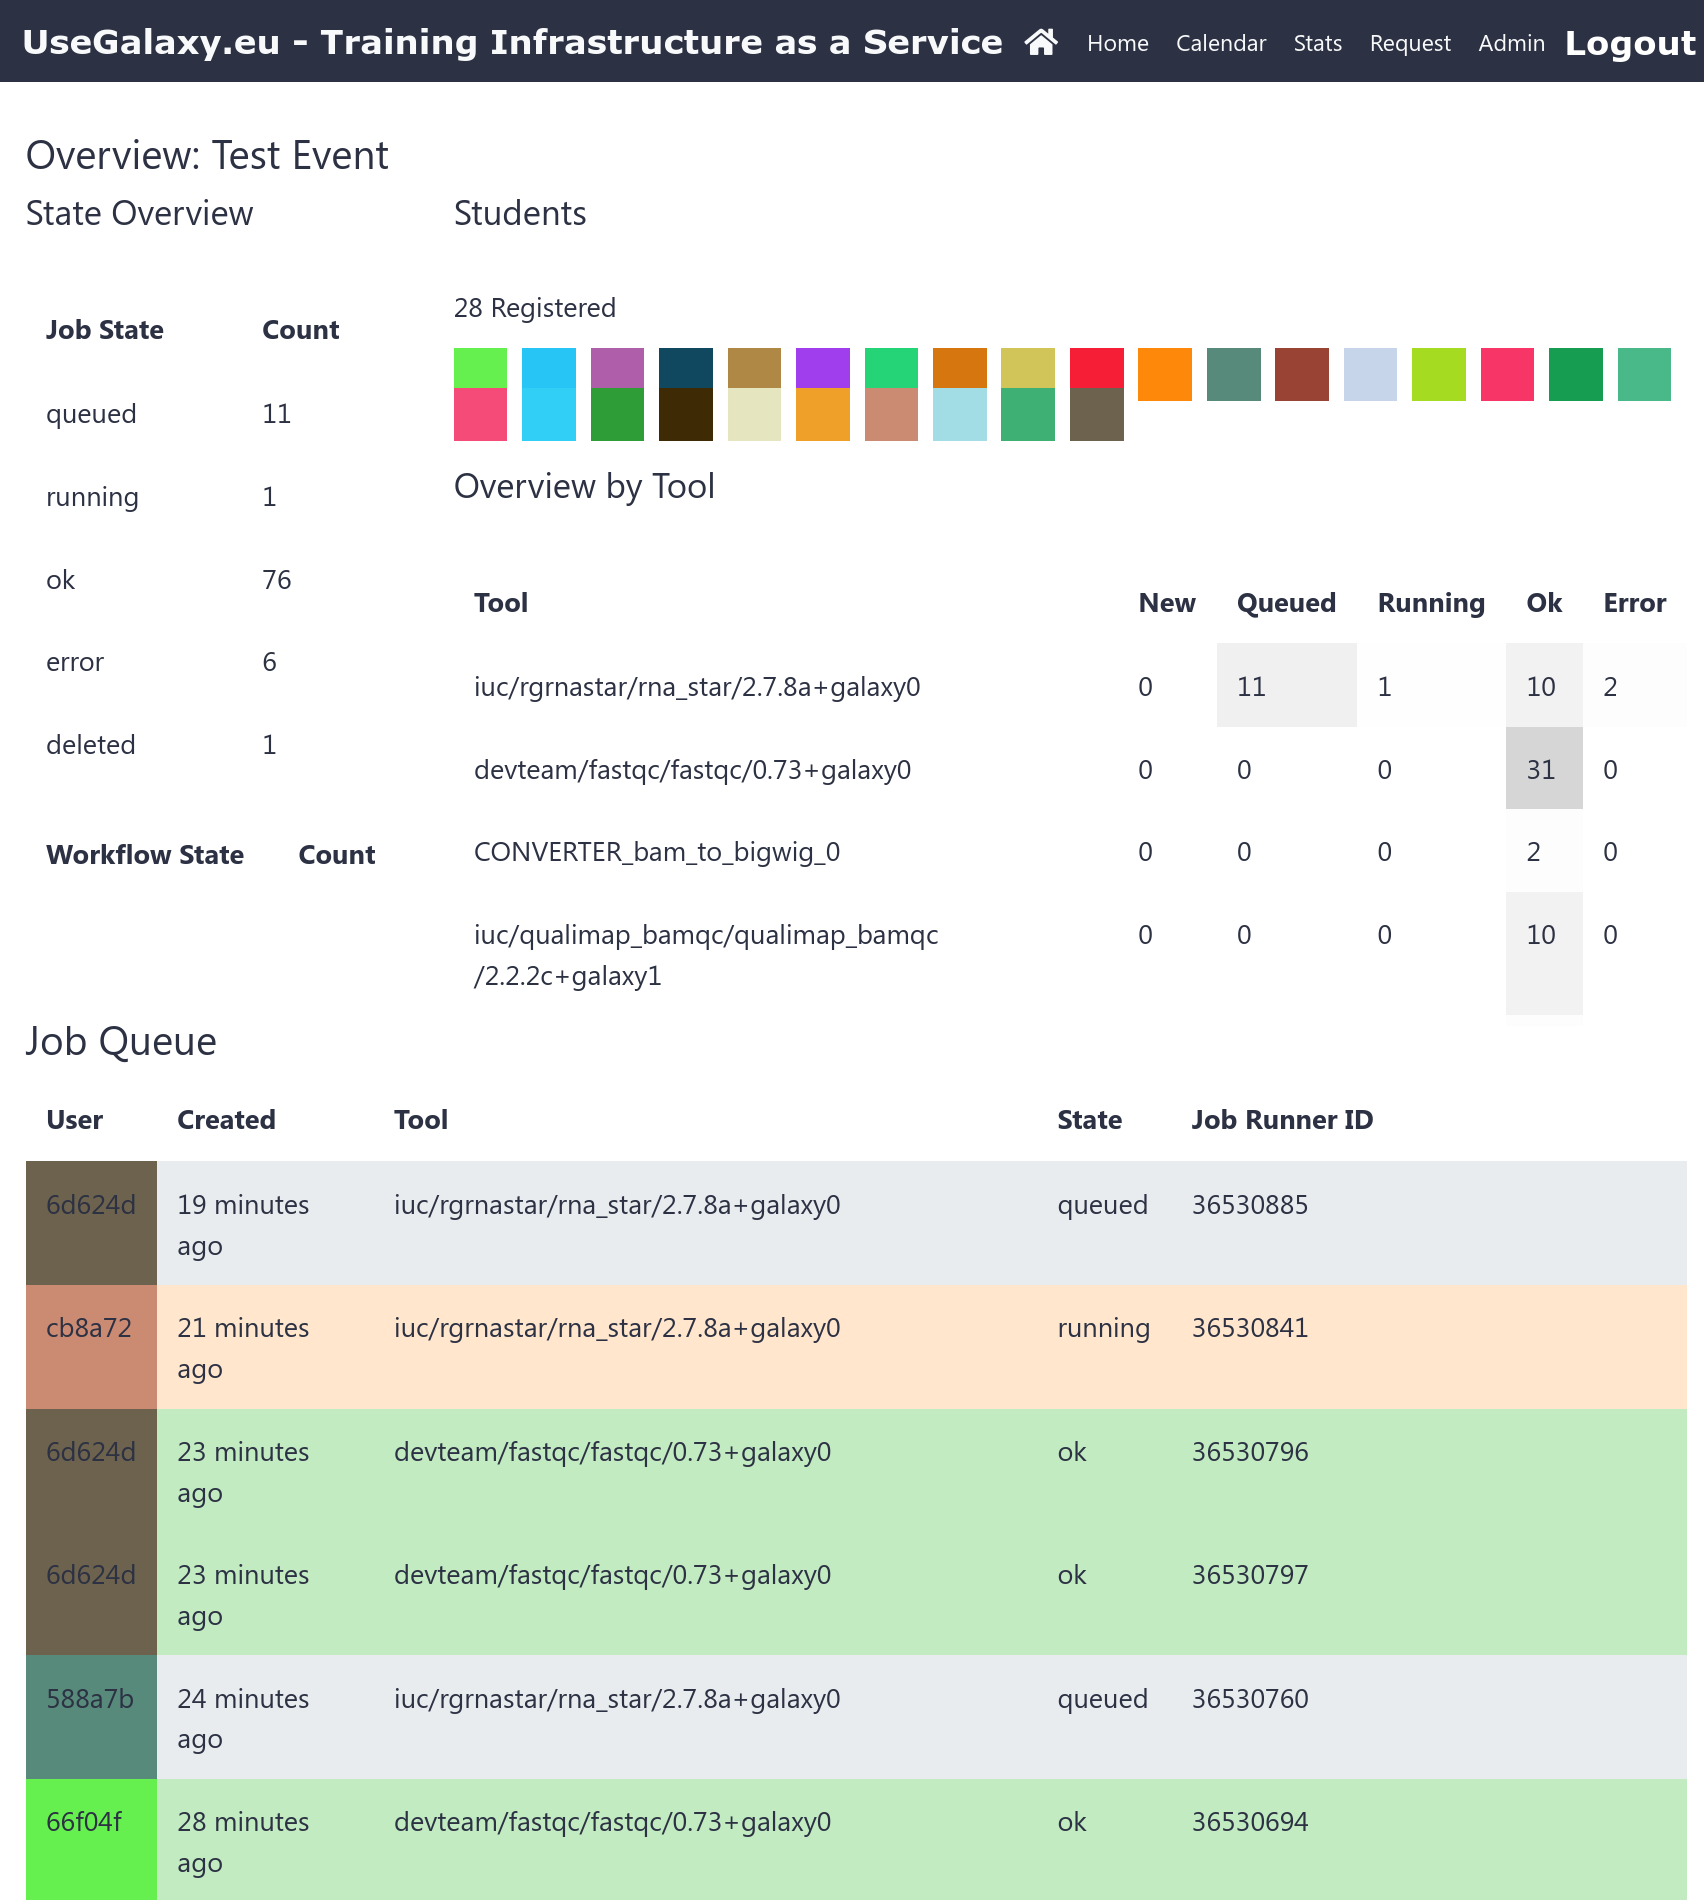
\includegraphics[width=\linewidth]{images/dashboard.png}
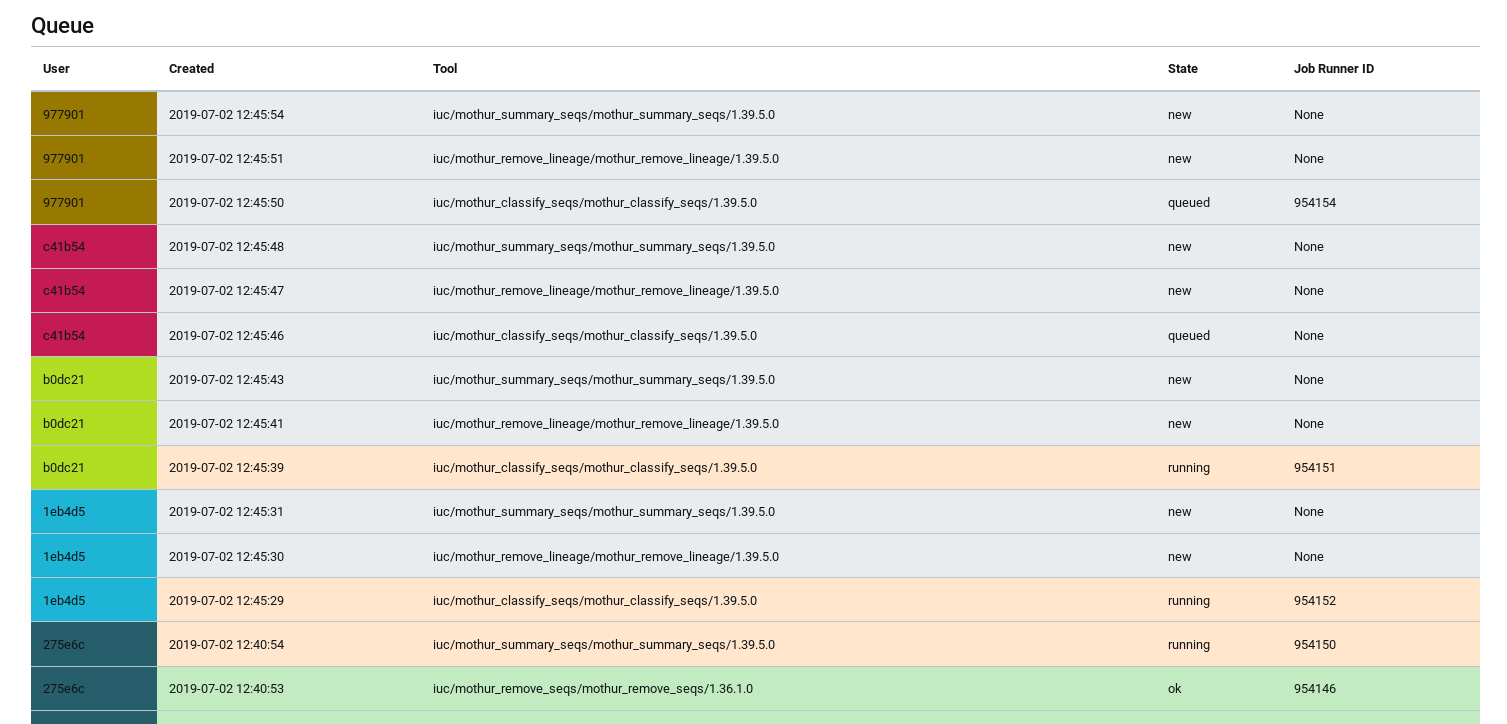
\includegraphics[width=\linewidth]{images/queue.png}
\caption{The top of the training dashboard page shows the status of the jobs in the past hours. A heatmap of the tools which were run indiciates if everything is running smoothly or if there is anything the trainer should look into. As learners follow along and run different tools, these show up immediately, allowing instructors to identify if everyone has started or finished a specific step. The bottom image shows the rest of the training dashboard, which lists jobs that were run chronologically, colour coded first by user, and second by the job status. Randomized colours and identifiers are used to protect user privacy, as we wanted dashboards to be easily shareable to course members.}\label{figure:dashboard}
\end{figure}

To create TIaaS, we implemented a web service, and separate job scheduling rules, which function together to present a private queue for users in specific Galaxy user groups. Event organizers register their course using a form in the TIaaS web service, where they are asked to provide information about the training  materials they will use, and the expected number of participants. Galaxy administrators review these requests, using information about the class size, the tools used in the training materials, as well as the resource allocations of those tools on the infrastructure, to estimate the required compute resources.

If resources are available and any other site-specific criteria are met, the training can then be approved. Next, administrators (optionally) deploy additional private compute resources, or re-allocate existing resources, in a local compute environment and attach them to their existing Galaxy scheduling, via the job scheduling rules. Administrators can then provide instructors with a URL such as \url{https://usegalaxy.eu/join-training/test}, and the instructor can then in turn provide to their learners. When training participants access the URL, they are registered in the TIaaS system, without the service administrator or trainers needing to be aware of users identities to aid in privacy protection\footnote{Local deployments can choose to disable that, e.g. for Galaxies deployed within a university or highschool where attendee privacy is not a requirement.}. The job scheduler, once aware of the training group, will place any job run by someone in that training onto the private training nodes (Figure \ref{figure:queue}).

\begin{figure}[bt!]
\centering
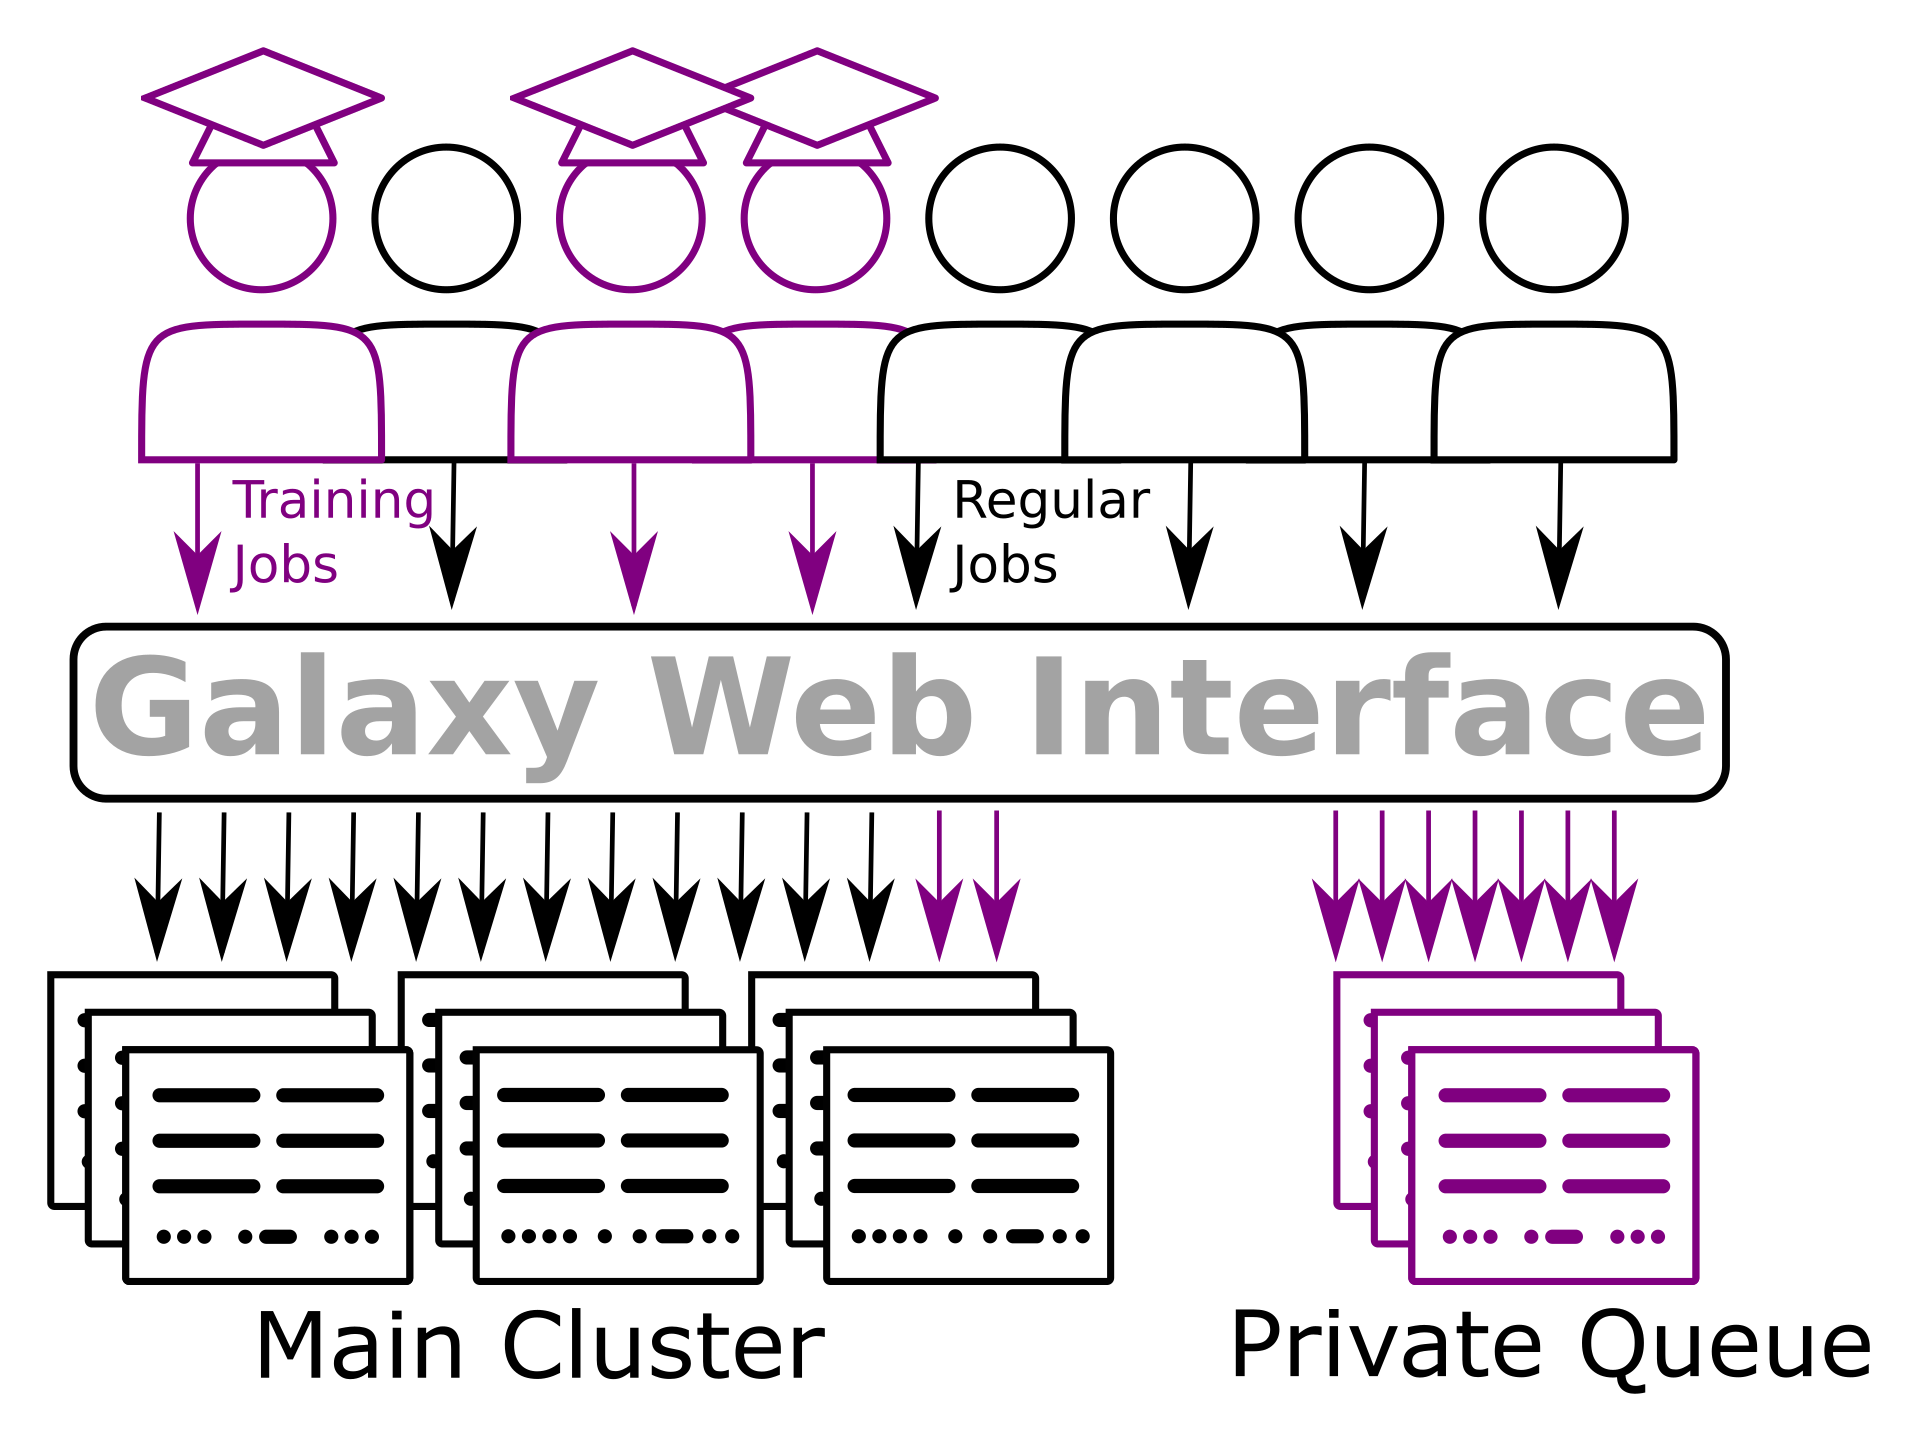
\includegraphics[width=\linewidth]{images/rules.png}
\caption{Schematic of the idealised TIaaS queuing system. Jobs are processed by the same Galaxy server, but when those jobs come from users in the training group, they receive special handling. These jobs are allowed to run on the private training resources (purple). If the training resource is full, these jobs can spill over to the main queue if necessary.}\label{figure:queue}
\end{figure}

The course dashboard, visualising the progress of participants (Figure \ref{figure:dashboard}), has significantly improved the ability of instructors to monitor progress of the learners, especially situations involving remote participants. The dashboard provides instantaneous, aggregated, and pseudonymised feedback for the instructors into how the learners are progressing. It has also simplified progress tracking in hybrid trainings, which were previously very labour intensive due to the necessity of maintaining insight into potential issues across multiple locations. This required per-site dedicated helpers to regularly provide up-to-date communication to the main instructor on how participants are progressing. With the training dashboard however, the instructor is no longer dependent solely on this communication from the satellite locations, but can monitor progress via the dashboard in real-time, and spot problems as they arise. Instructors can see which analysis steps are completed successfully by how many of the participants, and whenever there are many issues (e.g. failed jobs), they know that they might need to pause or explain the step in more detail.

\subsubsection{Usage}
Since the introduction of TIaaS in July 2018, it has seen nearly constant use with more than $>$360 trainings occurring on the platform, all across the world (Figure \ref{figure:graphs}).
Everything from one-day workshops for bioinformaticians to multi-month courses for highschool students have been hosted by TIaaS and UseGalaxy.eu, covering topics as wide-ranging as SARS-CoV-2 analysis, Imaging, Proteomics, and Machine Learning. All of this infrastructure has been provided for free across the big three Galaxies (EU, Americas, Australia), in thanks to the various grants supporting their associated Galaxy deployments.

\begin{figure}[bt!]
\centering
	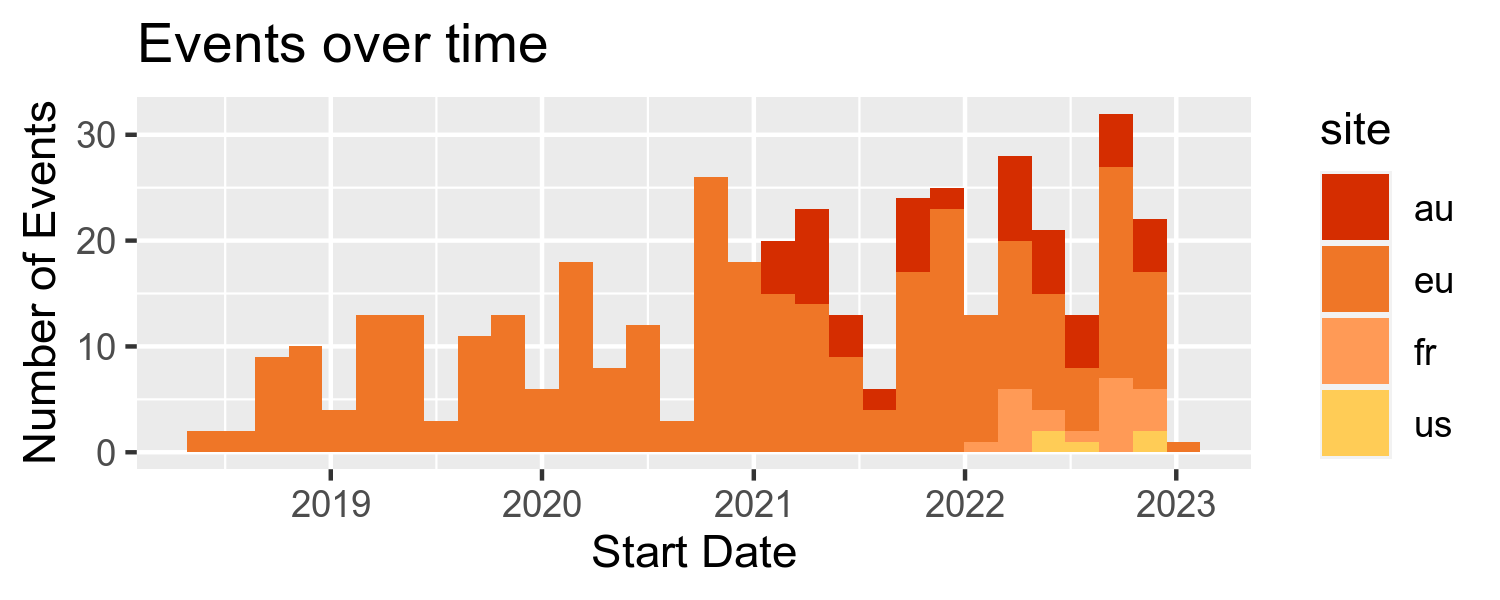
\includegraphics[width=\linewidth]{event-starts.png}
	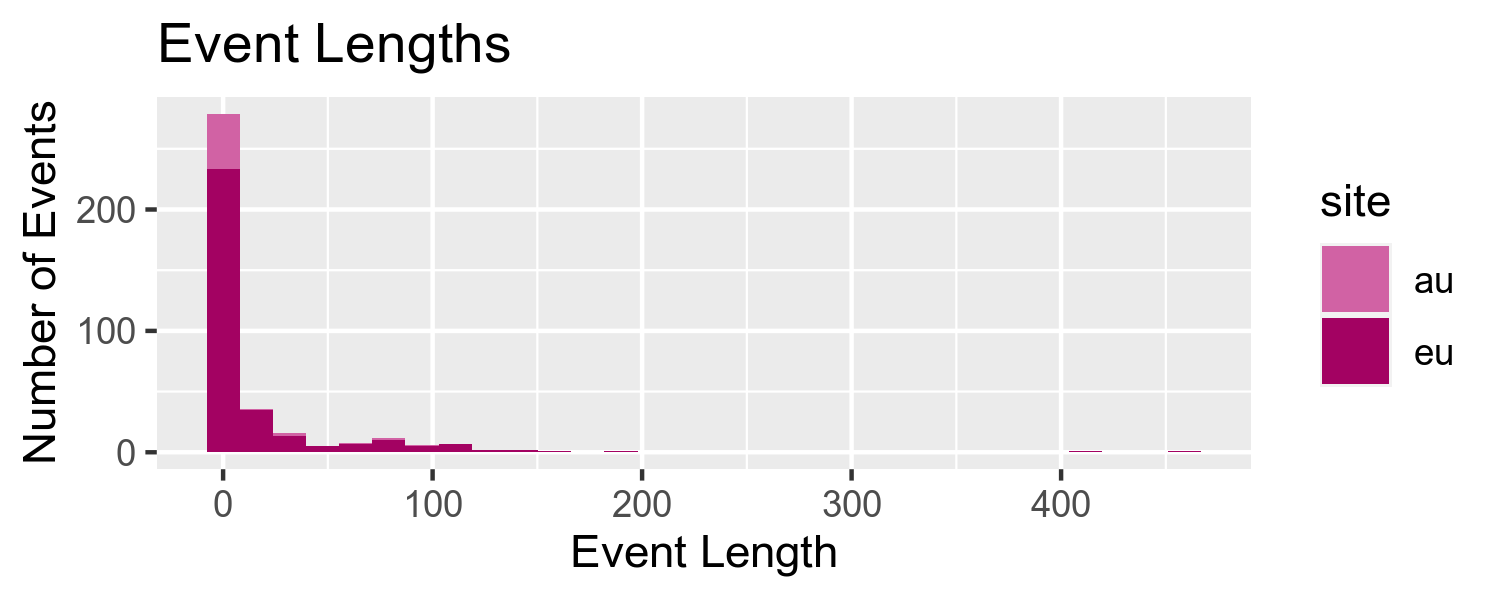
\includegraphics[width=\linewidth]{event-lengths.png}
	\caption{Since it's introduction is has grown into a well used service over the past four years. There have been more than 360 training events, spread across two primary instances that are very involved in training. Event length distribution is extremely heavily skewed to very short events, with a long tail of semester-long courses using the platform.}\label{figure:graphs}
\end{figure}

Class sizes have ranged considerably, from the median of 25 participants (std. dev 164) to a maximum of 2000 registrants for a fully asynchronous (self-paced) course. Most courses were short training events with a median of two days, however some ran for multiple months like a number of highschool courses which used TIaaS over the entire semester. The variability in administrator deployments of TIaaS can allow it to accommodate a wide range of teaching scenarios; for some courses large resources may be allocated like the Galaxy Community Conferences where the big three Galaxies configured TIaaS with considerable resources to permit local and remote synchronous training, all the way to semester long courses which may not necessitate a large amount of resources.

\section{Methods}

\subsection{Implementation}
TIaaS was written in Python with the Django framework. It has been designed from the start to have a very limited scope: provide a form to register events, an approval flow for administrators, management of user groups and roles in the Galaxy database, and the status dashboard.

For instructors a form is provided (\texttt{/tiaas/new}) which permits them to register a new training event. When submitted, this is stored in the associated database. Administrators can view the requested training events and approve or reject them using the built in Django admin interface. When users visit their their training url (\texttt{/join-training/<id>}) the system accesses their Galaxy session cookie, which is present as TIaaS is deployed at a path below Galaxy, and decodes it. They are automatically registered as part of a Galaxy group named after the training (e.g. \texttt{training-<id>}) which is created on demand.

When visiting the dashboard (Figure \ref{figure:dashboard}), the training ID is extracted from the URL (e.g. ``test'' from \url{https://usegalaxy.eu/join-training/test/status}), and all non-terminal jobs, in the past 1-6 hours, from those users are presented in a pseudonymised manner.

\subsubsection{Overview Pages}
Information over the status of the TIaaS system is provided via the interface. The calendar page made with Vue.js (e.g. \url{https://usegalaxy.eu/tiaas/calendar/}) shows upcoming training events, as well as their details if one is logged in as a TIaaS administrator. This is complemented by the stats view (e.g. \url{https://usegalaxy.eu/tiaas/stats/}) which shows overall system statistics giving funding agencies and staff a live view of the impact their service is having on the community and world.

\subsubsection{Scheduling}
When a job is submitted by a user in a training group, the Galaxy instance's job scheduling system system reads the user's groups and roles, and if any of these include something prefixed with \texttt{training-}, then this is converted to a job scheduler specific requirement string (Figure \ref{code:scheduler}, \ref{code:tpv}). Ideally these are scheduled to prefer training nodes, and spill over to the main queue if training nodes are full, but this feature is dependant on specific scheduler capabilities. 

In HTCondor this can be accomplished by preventing regular jobs from running on training nodes, and then allowing training jobs to run on training nodes, and preferring those nodes via configuration like in Figure \ref{code:condorprefer}.

Slurm, in contrast, requires either using TPV's notion of machine tags to separate jobs onto those specific, or selection a partition with \texttt{--partition=training-nld}

\begin{figure}[!ht]
\centering
\begin{lstlisting}[frame=single]  % Start your code-block
# HTCondor
Requirements=(GalaxyGroup == training-nld) || (GalaxyGroup == training-aus)
+Group="training-aus, training-nld"
\end{lstlisting}
\caption{HTCondor configuration to prefer specific training nodes.\label{code:condorprefer}}
\end{figure}



\begin{figure}[!ht]
\centering
\begin{lstlisting}[frame=single,language=Python]  % Start your code-block
def queue_job(job, user):
    job.cluster = 'main'

    if inTrainingGroup(user):
        training = getTrainingGroup(user)
        job.cluster = training

    return job
\end{lstlisting}
\caption{Python pseudocode representing how TIaaS jobs are typically processed and allocated to a private queue.\label{code:scheduler}}
\end{figure}

Or, rewritten for the modern Total Perspective Vortex (TPV) scheduler that is in place at the big three UseGalaxy servers:

\begin{figure}[!ht]
\centering
\begin{lstlisting}[frame=single,language=ini]  % Start your code-block
roles:
  training.*:
    scheduling:
      require:
        - training
\end{lstlisting}
\caption{YAML formatted TPV configuration that schedules jobs coming from users with a training role to any machines labelled as training nodes.\label{code:tpv}}
\end{figure}

\subsection{Deploying}
As the Galaxy community has largely settled on Ansible for deployment of Galaxy, and related components, an Ansible role was produced for deploying the TIaaS Service. A few known deployments make their configuration public, and we can see the differences: one the motivating factor in TIaaS' design was such flexibility. \emph{Galaxy Europe} uses it with HTCondor, and job rules that allow spill over to the main cluster, new machines are brought up in an OpenStack cluster specifically for training events and destroyed afterwards. Each Machine is tagged with an HTCondor attribute indicating which training it belongs to, and the job rules\footnote{Visible in \url{https://github.com/usegalaxy-eu/infrastructure-playbook/pull/447/files}} use that to enable access to those machines, and a preference for them. \emph{Galaxy Australia} has a separate ``training cluster'' in their OpenStack deployment, and route all training jobs to the single shared cluster\footnote{Visible at \url{https://github.com/cat-bro/infrastructure/blob/81ce910b74aafb333085e5fbc42fe5b37c3b4cab/files/galaxy/dynamic_job_rules/pawsey/total_perspective_vortex/roles.yml}}. \emph{Galaxy Main} takes a different approach, lacking additional clusters but having an excellent queuing system, they artificially limit the runtime, memory, and CPU resources allocated to users running jobs within a TIaaS group. \emph{Avans Hogeschool} uses TIaaS in an internal Galaxy where they provide no preferential treatment, and just use the dashboard to observe students.

\section{Availability of source code and requirements}

\begin{itemize}
\item Project name: ~Training Infrastructure as a Service
\item GitHub repository:~\url{https://github.com/galaxyproject/tiaas2/}
\item Admin Training Manual: ~\url{https://training.galaxyproject.org/training-material/topics/admin/tutorials/tiaas/tutorial.html}
\item Teacher Training Manual: ~\url{https://training.galaxyproject.org/training-material/topics/instructors/tutorials/setup-tiaas-for-training/tutorial.html}
\item Operating system(s): ~Unix
\item Other requirements: ~Galaxy version 18.01 or higher
\item License: ~GNU AGPL-3.0
\end{itemize}

\section{Availability of supporting data and materials}
All code is open source and available on GitHub (https://github.com/galaxyproject/tiaas2).

\section{Declarations}

\subsection{List of abbreviations}
\begin{itemize}
\item TIaaS: Training Infrastructure as a Service
\end{itemize}


\subsection{Competing Interests}
The authors declare that they have no competing interests.

\subsection{Funding}
This project was made possible with the support of the Albert Ludwig University of Freiburg.
The work is in part funded by Collaborative Research Centre 992 Medical Epigenetics (DFG grant SFB 992/1 2012) and German Federal Ministry of Education and Research (BMBF grants 031 A538A/A538C RBC and 031L0101B/031L0101C de.NBI-epi). The article processing charge was funded by the Baden-Württemberg Ministry of Science, Research and Art and the University of Freiburg in the funding programme Open Access Publishing.

This project is funded with the support of the Erasmus+ programme of the European Union (Grant 2020-1-NL01-KA203-064717).

\subsection{Author's Contributions}
HR and BG conceived of the presented idea. HR carried out the implementation. Significant improvements were later made by CH, JD, and AB. HR, BG, SG, NC, AB, and GC managed deployments of the software in production environment and bug detection. BSS and JHJ were responsible for user support and many suggested improvements. HR and BG contributed to the writing of the manuscript. BG and AS supervised HR.

\section{Acknowledgements}
The authors would like to thank the Galaxy community for their enthusiasm for this project, and their feedback on each iteration.

%% Specify your .bib file name here, without the extension
\bibliography{paper-refs}

\end{document}
